\documentclass[11pt]{article}
%\documentclass[prb,11pt]{revtex4-1}
\usepackage{multicol}
\usepackage{shortvrb}
\usepackage{url}
\usepackage{graphicx}
\usepackage{braket}
%\usepackage[hypcap]{caption}
\usepackage{capt-of}
\usepackage{amsmath}
\usepackage{mathdots}
\usepackage{fullpage}
\usepackage[font=small,labelfont=bf]{caption}
\usepackage{cite}
%\usepackage{hyperref}
\newcommand{\unit}[1]{\ensuremath{\, \mathrm{#1}}}
\usepackage{siunitx}
\usepackage{multicol}
\usepackage{cite}
\DeclareMathOperator{\Tr}{Tr}
%Gummi|061|=)

\title{Thesis}
\date{\today}
\author{Luka Milic}
\begin{document}

\begin{titlepage}
\sffamily
  
\includegraphics[scale=0.7]{img/uob-logo.png}\hfill
  \LARGE DEPARTMENT OF PHYSICS \\
  \begin{center}
    FINAL YEAR PROJECT, DISSERTATION OR\\
    PHYSICS EDUCATION REPORT
  \end{center} 

  \large
  \begin{tabular}[t]{|l|p{9cm}|}
    \hline
    NAME: & Luka Milic \\ \hline
    DEGREE COURSE: & Mathematics and Physics (MSci)\\ \hline
    PROJECT TITLE: & Entanglement of photons pairs generated in silicon ring resonators \\ \hline
    YEAR OF SUBMISSION: & 2015\\ \hline
    SUPERVISOR: & Damien Bonneau, Josh Silverstone and Mark Thompson\\ \hline
    NUMBER OF WORDS: & 282 (exclude appendices, references, captions and abstract)\\ \hline
  \end{tabular}
  \\[1.5cm]
  \begin{center}
    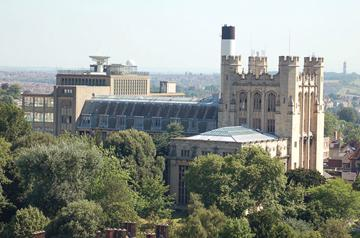
\includegraphics[scale=1]{img/physics-building.jpg}
  \end{center}
\end{titlepage}
\renewcommand{\abstractname}{Acknowledgements}
\newpage
\begin{abstract}
 Thanks Lizzy, Daminen, Josh, Mark, Raf, Imad, Phil, Mark. The NSQI, CQP Admin team.
\end{abstract}
\newpage
\tableofcontents
\newpage
\newpage
\section{Introduction}
The endeavour to build a quantum computer holds the promise of solving computational problems which are currently intractable on classical computers. A particularly promising paradigm for this is the linear optical quantum computer (LOQC) model which in theory allows for scalable universal quantum computation. Work on LOQC can be done using bulk optics components but this quickly becomes impractical when the experiments need to be scaled up to more qubits. Integrated photonics is a solution to this problem and allows for experiments a much higher component density, an essential ingredient to scalable quantum computing. General optical circuits can be implemented on such chips, popular materials are silicon-on-insulator (SOI) , lithium niobate and glass materials. Here we focus on SOI chips as they have many promising properties for the implementation of complex quantum optical circuits.

A key requirement for the full implementation of LOQC is a scalable, bright, deterministic and indistinguishable single photon source. Single photon sources in the SOI platform are typically made from the waveguide itself and use the spontaneous four-wave mixing which occurs in silicon due to the third order non-linearity to create a single photon pair. This report aims to develop a method of measuring the indistinguishably of the produced photons with a classical technique, exploiting stimulated four-wave mixing. This method collects a joint spectrum which is an estimation of the spectral shape of the two photons produced by the source. For a full description the Joint Spectral Amplitude JSA is the desired quantity, this is a full description of the wavefunction of the single photons emitted by the silicon ring resonators. However it is only within the scope of this work to measure the Joint Spectral Intensity, which is the absolute value squared the JSI. This gives an estimate of the JSA and allows to to upper bound the purity of the source.

The mission is therefore to develop a methodology to reconstruct these wavefunctions and hence engineer indistinguishable (high purity) single photon sources. In this work we performed such measurements on three SOI chips. The experimental work started with an initial proof of concept that one can collect joint spectrum data in the way desired. This was done on a chip supplied by Marc Sorel from Glassgow University. Then due to the fragility of these chip at high powers the experiment progressed to a chip manufactured by Toshiba. Finally in order to investigate a promising new material, amorphous silicon chip was used for experiments. 

In parallel techniques of analysing the output data are developed. Filtering techniques which remove noise are developed in order to make the data usable. A general framework is set out which aims to quantify the certainty in the measurements.

Finally we conclude that there is still much to be done in this area, proposing an outline for how to carry out effective measurements in the future.



\newpage
\section{Detailed Background and Theory}
\subsection{From Feynman to the linear optical quantum computer}
It was Richard Feynman in 1982\cite{feynman_simulating_1982} who first imagined it might be possible to efficiently simulate quantum systems with other quantum systems and hence end up doing computations that no classical computer could do in a reasonable (polynomial) time. The basic element of a quantum computer is the qubit, which can be written as
\begin{equation}
\ket{\psi}=\alpha \ket{0}+\beta\ket{1}
\end{equation}
this says the qubit is in a superposition of being in the $\ket{0}$ and $\ket{1}$ state at the same time, $\alpha$ and $\beta$ are the complex probability amplitudes. If we perform a measurement there is a $|\alpha|^2$ probability of measuring $\ket{0}$ and a $1-|\alpha|^2=|\beta|^2$ probability of measuring $\ket{1}$. This is a generalization of the classical bit, which can only ever be set to 0 or 1. With this added structure, quantum computers can in theory out perform classical computers in certain tasks such as factorisation \cite{shor_polynomial-time_1995}, meteorology \cite{toth_quantum_2014}, quantum chemistry\cite{georgescu_quantum_2014} and they can be used to establish communication systems secured by the laws of physics with quantum key distribution (QKD)\cite{zhang_reference-frame-independent_2014}.

With the exception of QKD none of these applications have yet been fully realised, in particular because not all of the criteria  \cite{divincenzo_quantum_1998} set out in 1998 by DiVincenzo for a universal quantum  computer have been met. These are:
\begin{itemize}
	\item A scalable physical system with well characterized
qubits
	\item The ability to initialize the state of the qubits to a
simple fiducial state, such as $\ket{000...}$
	\item Long relevant decoherence times, much longer than
the gate operation time
	\item A “universal” set of quantum gates
	\item A qubit-specific measurement capability
\end{itemize}

This work aims to make some progress on the first two criteria in the context of integrated optical quantum computers. Here we define qubits as photons, with $\ket{0}$ and $\ket{1}$ denoting the path a photon takes through a linear optical quantum circuit (LOQC). Figure \ref{loqc} shows how a LOQC fits into a wider context, with single photon sources supplying qubits, single photon detectors reading out the results of the computations and a classical computer to feedback the the results into the circuit. To discuss the two criteria further we first introduce single photon sources.

\begingroup
    \centering  
    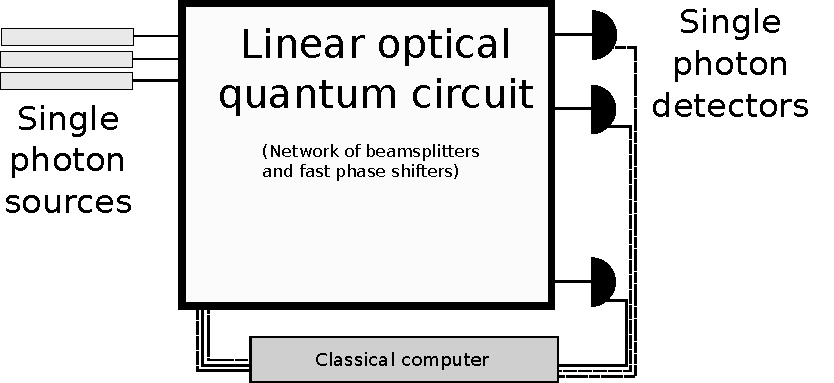
\includegraphics[width=12cm]{img/theory/loqc.pdf}
    \captionof{figure}{A conceptual outline of the architecture of a optical quantum computer, single photon sources supply the qubits which are fed into reconfigurable circuits which are altered depending on the pattern of photons detected at the detectors. }
     \vspace{3pt} \label{loqc}
\endgroup

%We focus in on the first two criteria from DiVencenzo \cite{divincenzo_physical_2000}, "A scalable system with well characterized qubits", which in the context of figure \ref{loqc} refers to the single photon sources. This criteria tell us that our photons must have no degrees of freedom apart from one which allows the photons to act as qubits. This means each time a photon is generated it must have the identical spectral and phase characteristics, in other words it must be in a pure state and not in statistical mixture of states.
%A particular way in which the photons might be different is in their energy and phase distribution. This is described by their Joint Spectral Amplitude (JSA), this along with the Joint Spectral Intensity (JSI) which is the absolute value squared of the JSA is the focus of this work. By measuring the JSI we can begin to explore how existing methods of generating single photons are performing.



\subsection{Generating single photons}
The previous section motivated the the need for a single photon source, we first look at the history and then focus on one promising source, the ring resonator on a silicon photonic chip.

The ideal single photon source would produce exactly one photon when triggered in a pure quantum state, which means it is in a state superposition of all of its spectral components rather than a statistical mixture. This is happens if the temporal shape is the same as the Fourier transform of its spectrum \cite{uren_generation_2007}. Such a perfect source does not yet exist. We can divide existing sources into two categories deterministic and non-deterministic. The first kind are typically small single atom or molecule systems, which respond deterministically to some kind of impulse. For example a single atom two level system can be excited by a laser pulse into the upper level, it will then emit a photon of some fixed energy after some relaxation time. 


In the past these experiments have typically been performed with bulk optics meaning that each element is fixed to a large optical work bench, carefully aligned with the next element and with the light travelling in the air in between. These experiments take up a lot of lab space and quickly encounter resource constraints if they try to become too complex. A solution to this is to translate each of the components onto a integrated chip, where far less alignment is needed, the important devices always maintain the same separation and most importantly vastly more complicated circuits can be designed. This is of course essential to the endeavour of using LOQC's to perform complex quantum operations. Note again Divencenzo's first criteria, referring to scalability, integrating photonics onto chips makes a lot of progress on this front.

Photonics can be integrated onto chips of various materials, typical choices are glass, lithium niobate and silicon. Here we focus on silicon, it has the advantage that advanced fabrication techniques exist due to the multi-billion dollar semiconductor industry. Two types of silicon are used, the first is the standard silicon with its periodic lattice structure and the second is amorphous silcion which forms a random network structure. Amorphous silicon could potentially solve problems with standard silicon such as two photon absorption and subsequent free carrier absorption which is known to be detrimental to single photon sources.

On chip single photon sources on silicon have been studied [, , , ] and shown to be a promising platform. Currently two ways of producing photons are employed. The first way employs large spools of waveguide towards the start of the circuit into which a intense laser beam (referred to as the pump) is injected and due to non-linear processes single photons are produced. This happens because silicon has a $\chi^{(3)}$ non-linearity and so a small amount of frequency conversion occurs. The process called spontaneous four wave mixing (SFWM) takes two pump photons $\omega_{p_1}$, $\omega_{p_2}$ and converts them into a signal $\omega_s$ and  $\omega_i$ idler according to the following energy conservation equation.

\begin{equation} \label{energyConservation}
\omega_{p_1}+\omega_{p_2}=\omega_s+\omega_i
\end{equation}

This equation works in general, for a laser beam with only one frequency we write $2\omega_p=\omega_s+\omega_i$. An upshot of producing two photons is that this is a heralded single photon source, meaning it is possible to know when you've generated a photon by using, for example, the idler as your herald and the signal as the heralded photon. 

Now this process occurs in the waveguide due to the high intensity beam, a second alternative way to control the generation of the single photons is to create a cavity into which the beam can couple and produce single photon pairs (signal and idlers) with a high probability. The cavity which we focus on is the ring resonator, a structure with interesting spectral properties which can be manipulated to increase the purity of the generated photons. 


%Quantum optics experiments were first conducted in bulk optics \cite{burnham_observation_1970} and since then they have allowed for the development of a large body of physics, some of which have pushed the frontiers of fundamental physics. Such experiments have certain basic elements in common such as beam splitters, filters, polarisation controllers, phase shifters, etc. With these elements occupying a fair amount of space in a lab there is a practical size limit on what can be done, hence there has been a recent push into compressing such optical experiments onto a single photonic chip. Each of the optical elements described previously can be implemented onto such chips. The free space propagation of light is replaced by waveguides etched onto materials such as silicon, lithium niobate or glass. Beam splitters and couplers are implemented by running two waveguides close enough to each other so that light can couple between them via their evanescent fields. Filters are implemented as ring resonators which are circular cavaties into which only certain wavelengths of light will resonate and hence be filtered. Phase shifts can be induced by heating small portions of the chip with an electrical probe.

%Here we focus in on a particular element, the ring resonator etched onto silicon photonic devices. Silicon is an attractive material primarily due to the already established microchip industry which can produce highly precise structures at the nanoscale on the back of decades of demand for faster and smaller computing devices. Furthermore silicon has a high $\chi^{(3)}$ non-linearity enabling frequency conversion and hence the implementation of a single photon source.

\subsection{Four wave mixing in silicon waveguides}
Here we motivate some of the theoretical background to four wave mixing in order to arrive at why ring resonators can be used to better exploit the process. 

Waves travel through non-linear materials according to the non-linear wave equation:
\begin{equation}
\nabla^2 \mathbf{E} - \frac{n^2}{c^2}\frac{\partial^2}{\partial t^2}\mathbf{E}
= \frac{1}{\varepsilon_0 c^2}\frac{\partial^2}{\partial t^2}\mathbf{P}^{NL}
\end{equation}

\begin{equation} \label{polEqn}
\mathbf{P}^{NL} =\sum^\infty_{n=0} \epsilon_0\chi^{(n)}\mathbf{E}^n(\mathbf{x	},t)
\end{equation}

Where $\mathbf{P}^{NL}$ accounts of the non-linear response of the material, $\mathbf{E}(\mathbf{x},t)$ is the electric field . In silicon the predominant non-linear effect comes from the $\chi^{(3)}$ term, as this is a third order term, it enables wave mixing processes, a quick intuition for this can be gained by inputting into $ \epsilon_0\chi^{(3)}\mathbf{E}^3(t)$ a super position of two waves:


\begin{equation}
\mathbf{E}(t)=E_s\cos(\omega_st)+E_p\cos(\omega_pt)
\end{equation}
\noindent
The result is proportional to:
\begin{align}
&E_p E_s^2 \cos ((2 {\omega_s}-{\omega_p})t)+E_p E_s^2 \cos ((2 {\omega_s}+{\omega_p})t)\\
&+ E_p^2 E_s \cos ((2{\omega_p}-{\omega_s})t)+ E_p^2 E_s \cos (({\omega_s}+2 \omega_p)t) + h.t.
\end{align}
\noindent
Where $h.t.$ are the harmonic terms, such as $E_1^3\cos(3\omega_p t)$ which are we aren't interested in here. We notice that four new frequencies are generated, in experiments one typically denotes $E_p$ the pump and $E_s$ the signal, with $E_p >> E_s$. Due to the pump beam being of higher intensity we are left with two processes:
\begin{equation}
	2\omega_p+\omega_s = \omega_i^{(1)}
\end{equation}
\begin{equation} \label{FWM}
	2\omega_p-\omega_s = \omega_i^{(2)}
\end{equation}
We call the resulting beam $\omega_i$ the idler. Now we take interest in the second process(equation \ref{FWM}) because this is one typically used in quantum optics to produce photon pairs for a single photon source. Rewriting it as $	2\omega_p = \omega_i+\omega_s$ and thinking of the classical waves as streams of photons we can see that two pump photons can be converted into signal and idler photons. This conversion is allowed due to vacuum fluctuations stimulating the process, these are very weak and so the efficiency of the process is also quite low.

Discussion of phase matching has been omitted, but it is enough to say that in order for the process to constructively interfere and hence satisfy the wave equations we must have $2\mathbf{k_p}=\mathbf{k_i}+\mathbf{k_s}$.


Now in order to take this process to the single photon level we must introduce a way to talk about photons at the quantum scale. Because of the Heisenberg uncertainty principle the number of photons at each energy level can be uncertain. Such states are described by a vector in fock space, for example a state where there are two photons in the first and third energy level would be written as:
\begin{equation}
	\ket{2020...}
\end{equation}
The state for the vacuum or in other words for no photons is written as:
\begin{equation}
	\ket{vac}=\ket{000...}
\end{equation}
Operators exist to create and annihilate photons.
\begin{align}
& a_i^{\dagger}\ket{n_1,...,n_i,...}=\sqrt{n_i+1}\ket{n_1,...,n_i+1,...} \\
& a_i\ket{n_1,...,n_i,...}=\sqrt{n_i}\ket{n_1,...,n_i-1,...} \\
\end{align}
With commutation relations $[a_i,a_j]=[a^{\dagger}_i,a^{\dagger}_j]=0$ and $[a_i,a^{\dagger}_j]=\delta_{ij}$

The non-linear hamiltonian that governs the spontaneous four wave mixing process in the waveguide is:

\begin{equation}
\hat H_{NL} = -\chi^{(3)}\int_\infty^\infty\int_\infty^\infty\int_\infty^\infty\int_\infty^\infty S(k_{p_s},k_{p_i},k_{p_1},k_{p_2})( a_{k_{p_i}}^{\dagger}a_{k_{s}}^{\dagger}a_{k_{p_1}}a_{k_{p_2}} + h.c.)dk_{p_s}dk_{p_i}dk_{p_1}dk_{p_2}
\end{equation}

%
\noindent
The linear vacuum hamiltonian is also involved:

\begin{equation}
\hat H_{L} = \int_\infty^\infty a_{k}^{\dagger}a_{k}dk
\end{equation}
\noindent
Adding these two up gives the overall hamiltonian $\hat H = \hat H_{L} + \hat H_{NL}$. The function $S(k_{p_s},k_{p_i},k_{p_1},k_{p_2})$ represents the coupling between the various frequencies. 

This general frame work applies to both straight waveguide and ring resonator production of photon pairs. There is a large amount of literature [,,,,] which describes how to use it to derive the resultant wavefunction, here we simply state the general result:
\begin{equation}
\ket{\psi_{out}}=\left [1 + \frac{\beta}{\sqrt{2}}\int dk_1dk_2\Phi(k_1,k_2)a_{k_1}^{\dagger}a_{k_2}^{\dagger} \right ]\ket{vac} \label{JSAWavefunct}
\end{equation}
This is called the biphoton wavefunction, the reason we omit the full theory is because this project focuses on measurement and anylsis of $\Phi$ rather than it's exact theoretical origin. The biphoton wavefunction encodes all of the information about how the photon pairs were produced that effects its spectral and phase distribution. This includes the pump spectrum, intensity, the geometry of the waveguide or cavity used for the process.

This function $\Phi(k_1,k_2)$ is called the joint spectral amplitude (JSA) and its absolute value squared is called the joint spectral intensity (JSI). Returning to DiVenceno's criteria we require that this function is of the form $\Phi(k_1,k_2)=f(k_1)g(k_2)$ to explain this we introduce some more quantum theory.

A two party system in quantum mechanics can be described generally as:

\begin{equation}
\ket{\psi} = \sum_{i,j}\alpha(i,j)\ket{i}_A\otimes\ket{j}_B 
\end{equation}
\noindent
This state can be a pure state, so that $\alpha(i,j)=f(i)g(j)$ and so
\begin{equation}
\ket{\psi} = \left (\sum_{i}f(i)\ket{i}_A \right ) \otimes \left (\sum_{j}g(j)\ket{j}_B \right )
\end{equation}
meaning that there is no way that a measurement which happens in system A can effect system B. Otherwise it is in an entangled state and the sub systems act as statistical mixtures. The same idea can be applied to the wavefunction in equation \ref{JSAWavefunct} to give:
\begin{equation}
\ket{\psi_{out}}=\left [1 + \frac{\beta}{\sqrt{2}}\int dk_1f(k_1)a_{k_1}^{\dagger} \int dk_2f(k_2)a_{k_2}^{\dagger} \right ]\ket{vac}
\end{equation}
Which now says, if you measure the first photon there is no way you can influence the second photon. For a heralded source this is vital, the process of heralding must not interfere with the heralded photon and in particular not in this way as here it would make the photon collapse randomly into one of its modes.




In order to talk about how pure or mixed a biphoton wavefunction, the JSA can be decomposed into a linear superposition of pure states. This is written as\cite{harder_optimized_2013}:
\begin{equation} \label{modes}
	\Phi(k_1,k_2) = \sum_i \lambda_if_i(k_1)g_i(k_2)
\end{equation}

With $\sum_i \lambda_i=1$. Now it is possible to assess the separability of such a JSA by choosing a metric to quantify how many terms  equation \ref{modes} has. A convenient one is the purity defined as: 

\begin{equation} \label{purityEqn}
	P = \sum_i \lambda_i^4
\end{equation}

For a totally seperable state where there is only one $\lambda$ coeffecient, $P=1$ and this is its maximum value. The minimum value of P is less well defined and depends on the dimension of the system , in particular 


%In a straight waveguide the function $\Phi(k_1,k_2)$ is particularly non separable. It's features are defined mainly by the energy conservation of equation \ref{energyConservation} and the width of the pump. To illustrate this example with take two illustrative approximations of 


\subsection{Ring Resonators}
Using ring resonators as a way to improve the separability of the JSA has been tried and found to work. Here we describe why it works and the general workings of a ring resonator, we then finally move onto discussing metrics to quantify this separability in terms of purity and schmidt number.


Ring resonators are one of many devices which can be found on optical circuits on chip. They are closed strips of waveguide, placed near enough to the waveguide carrying light so that light can evanescently couple inside, in other words they form a cavity. By setting up a simple experiment, where light passes by the resonator and the transmission is measured for varying wavelengths a spectrum characterising the ring can be obtained. An example of one is shown in figure \ref{ringResTrans}, periodic resonances are visible with a spacing called the free spectral range (FSR). The physical reason for the resonances is that when the input beam is an integer number of wavelengths of the circumference of the ring, a high amount of destructive interference occurs because the light picks up a $\pi$ phase shift from coupling across waveguides.

\begingroup
\centering
    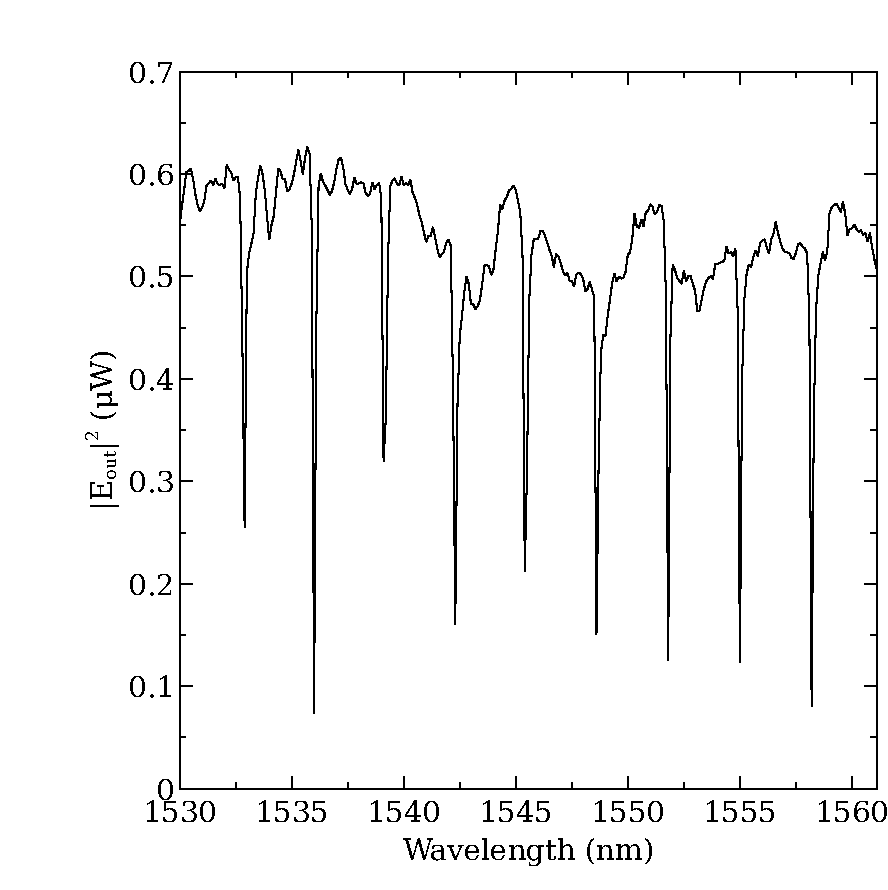
\includegraphics[width=9cm]{img/theory/ringTransmission.pdf}
\captionof{figure}{A typical ring resonator spectrum. } \label{ringResTrans}
\endgroup


A first order model for a ring resonator is called the linear ring model, this does not include non-linear effects which are discussed later but does allow for a good understanding of the different coupling modes a ring can be in. Following figure \ref{ringModel} $E_{in}$ is the injected laser beam and $E_{out}$ is the output light, where $|E_{out}|^2$ is what is typically measured in an experiment. $E_{1}$ is the field at the start of the ring and $E_2$ is the field at the end of the ring, by travelling around the ring some of the light is lost and a wavelength dependant phase relative to the input light is picked up.

\begingroup
\centering
    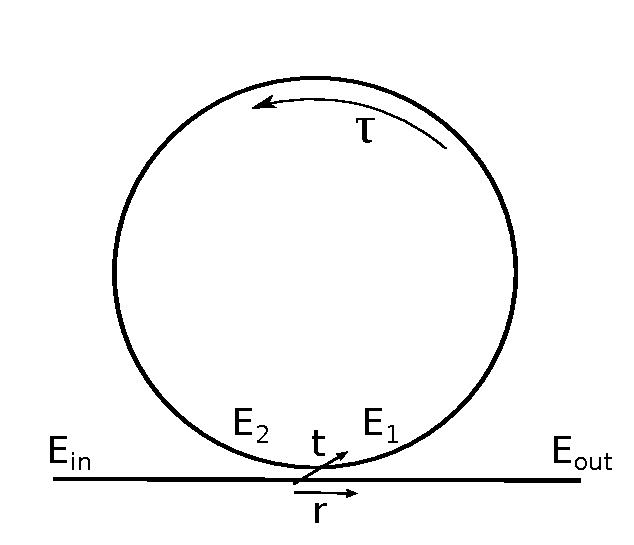
\includegraphics[width=9cm]{img/theory/ring.pdf} \label{ringModel}
\captionof{figure}{A simple but powerful model of a ring resonator. $E_{in}$ represents the input electrical field and $E_{out}$ is the field after interaction with the ring. $E_{1}$ is the field at the start of the ring and $E_{2}$ is this field with some loss due to propagation through the ring waveguide. We assume that the distance between $E_{out}$ and $E_{in}$ is much smaller than $E_{1}$ and $E_{2}$.}
\endgroup

We can model this system with the following set of linear equations, where $r$ is the fraction of light that passes by the coupling region and $t$ is the amount of light that couples across the coupler.
\begin{equation}
\begin{pmatrix}
E_{out} \\
E_{1} \\
\end{pmatrix}
=
\begin{pmatrix}
r & it \\
it & r \\
\end{pmatrix}
\begin{pmatrix}
E_{in} \\
E_{2} \\
\end{pmatrix}
\end{equation}
\noindent
With these matrices and also by noting that $E_2=\tau e^{i\theta}E_1$ is due to the ring causing a phase difference and some loss. We can derive expressions for each point in the system, for the full derivation refer to appendix \ref{ringResAppen}.

\begin{equation}
\left |\frac{E_{out}}{E_{0}}\right|^2=\frac{r^2-2r\tau\cos(\theta)+\tau^2}{1+r^2\tau^2-2r\tau cos(\theta)}
\end{equation}
\begin{equation}
\left|\frac{E_{1}}{E_{0}}\right |^2=\frac{1-r^2}{1+r^2\tau^2-2r\tau cos(\theta)}
\end{equation}
\begin{equation}
\left |\frac{E_{2}}{E_{0}}\right |^2=\tau^2\left|\frac{E_{1}}{E_{0}}\right |^2
\end{equation}

Where $\theta=kL=\frac{2\pi n_{eff}}{\lambda}L$. The analysis also finds the relation $r^2 = 1 - t^2$ , which is useful because it reduces the amount of variables we need to model the resonator.
\begingroup
    \centering  
    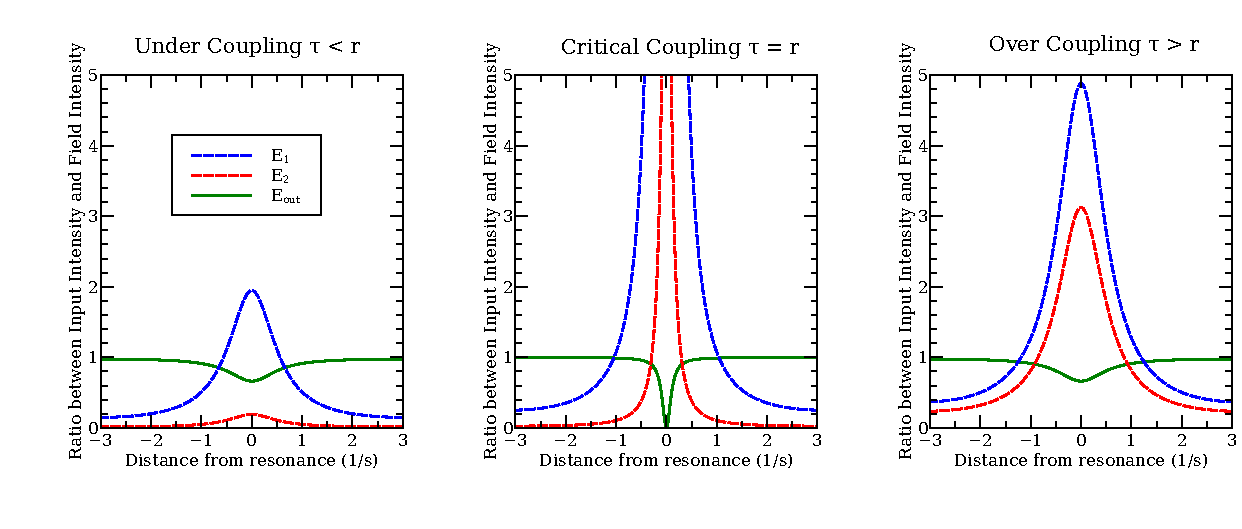
\includegraphics[width=17cm]{img/theory/coupling.pdf}
    \captionof{figure}{Notice how similar under and over coupling are to each other}
     \vspace{3pt} \label{coupling}
\endgroup

Figure \ref{coupling} shows the 3 main regimes that can be achieved by varying $r$ and $\tau$. The first is under-coupling, a typically undesirable set up where the ring loses more light than it recieves and hence performs low quality filtering. This looks identical to over-coupling where more light enters then ring than is lost. The fact that over and coupling look the same is an important point for later analysis, as when using a resonator as a single photon source, a small amount of over-coupling is desirable. 

Critical coupling occurs when the loss within the ring is balanced with the amount of light coupling in ($r=\tau$) this gives a spectrum with the highest quaility factory, where we define quality factor[REF] as:
%Jan Niehusmann, Andreas Vörckel, Peter H. Bolivar, Thorsten Wahlbrink, Wolfgang Henschel, and Heinrich Kurz. Ultrahigh-quality-factor silicon-on-insulator microringresonator. Opt. Lett.,29(24):2861–2863, December 2004.
\begin{equation}
Q \approx \frac{2\pi L n_{eff}}{-\lambda \ln{r\tau}}
\end{equation}

This metric is useful for comparing rings. 

\subsection{Bistability}
%The bistability effect is based on the carrier generation induced by two-photon absorption
It can be experimentally observed that injecting power into a ring resonator will cause changes in the spectral position and shape of the resonance. Typically in silicon ring resonators the more power in the ring the more the resonance position is red-shifted by the thermo-optic effect\cite{almeida_optical_2004-1}. A counter acting effect is carrier generation induced by two-photon absorption \cite{xu_carrier-induced_2006} which causes a blue-shift in the resonance position. This carrier generation process is much faster than the thermo-optic process so it more relevant to lasers with low repetition rates. 

The bistability effect is observed by changing the power injected into the ring resonator at a fixed wavelength. By steadily increasing the power of a monochromatic light source injected into the ring at a wavelength slightly higher than the resonance position $\lambda_{r}$ of the ring, $\lambda_{r}$ is increased (thermal effects dominate as the laser is a continuous wave and not pulsed). The shift in $\lambda_{r}$ accelerates as more light is coupled into the ring and transmission falls as more light is coupled into the ring. The system is now in a different and stable state (assuming the injected light is not discontinued). With a low intensity probe it is now possible to map out the new position and shape of the resonance.

By doing the reverse experiment with the input power decreasing a similar phenomena is observed, however the sudden accelerating changing in resonance position is seen for a different power due to the ring coming from a different stable state. A hysteresis loop can be observed.

Some knowledge of this effect is vital when planning experiments using high and variable powers, as one must take into account that the state of the ring is not fixed. Furthermore when automating equipment it may be vital to integrate knowledge of this into any scanning procedures. 

\subsection{Characterisation of quantum processes with classical techniques}
Marco \cite{helt_spontaneous_2010}
%Want to talk about some hamiltonians.

\subsection{Schmidt Rank and Purity}
%WHAT IS THE DIFFERENCE BETWEEN A GAUSSIAN BLUR AND BILINEAR INTERPOLATION?
% MATE THIS IS TOO MUCH

\subsection{Self phase modulation}
\section{Method}
\subsection{Coupling}
\subsection{Bistability}
\subsection{Joint Spectrum}
\subsection{$g^{(2)}(0)$}
\section{Results}
\subsection{Glassgow}
\subsection{Toshiba}
\subsection{a-Si}
\section{Discussion}
\section{Conclusion}
%\section{Lit Plan}
%READ THIS: \cite{jalali_silicon_2006}
%\bibliographystyle{unsrt}
\bibliographystyle{unsrt}
\bibliography{bibfile}
\newpage
\appendix 
\section{Schmidt Number}
\label{schmidtAppendix}
\subsection{Definition}
Here we recall some quantum mechanics in order to derive a way to find the purity of experimental data. Starting with some arbitrary state $\psi$:
\begin{align}
|\psi \rangle &= \sum_{i,j}\alpha(i,j)|i\rangle_A\otimes|j\rangle_B 
\end{align}
The schimdt number $K$ of this state measures the degree of entanglement. If $K=1$ then you can find $|\psi \rangle  = |\xi \rangle\otimes |\eta \rangle$ and for $K>1$ you can find: 
\begin{align}
|\psi \rangle &=\sum_{i} r_i|\xi_i \rangle_A\otimes |\eta_i \rangle_B
\end{align}
An expression for $K$ can be found using the density matrix for $\psi$:
\begin{align}
\rho_{AB} &=|\psi \rangle \langle\psi| = \sum_{i,j,k,l}\alpha(i,j)\alpha^*(k,l)|i\rangle\langle k| \otimes|j\rangle \langle l| \\
\rho_{A} &=\Tr_B(\rho_{AB}) = \sum_{i,j,k}\alpha(i,j)\alpha^*(k,j)|i\rangle \langle k|  \\
\rho_{A}^2 &= \sum_{i',j',k'}\sum_{i,j,k}\alpha(i,j)\alpha(k,j)\alpha^*(i',j')\alpha^*(k',j')|i\rangle \langle k|i'\rangle \langle k'|  \\
&= \sum_{j',k'}\sum_{i,j,k}\alpha(i,j)\alpha^*(k,j)\alpha(k,j')\alpha^*(k',j')|i\rangle \langle k'|  \\
\Tr_A(\rho_{A}^2)&= \sum_{i,j,k,j'}\alpha(i,j)\alpha^*(k,j)\alpha(k,j')\alpha^*(i,j')  \\
\end{align}
For a unentangled $\psi$ we know that $\Tr_A(\rho_{A}^2)=1$ For $\psi$ entangled this will be smaller than 1 (proof comes from the property of the density operator that its eigenvalues are all smaller than 1). This fits the definition of the purity of a quantum state hence we can write:
\begin{align} \label{theShit}
P = \frac{1}{K}&= \sum_{i,j,k,l}\alpha(i,j)\alpha^*(k,j)\alpha(k,l)\alpha^*(i,l)
\end{align}
\subsection{Calculation from experimental data}
\subsubsection{Trace method}
In the lab we can measure $|\phi(\omega_1,\omega_2)|^2$, here we outline how to extract the schimdt number from this set of values. Taking the positive square root of the matrix of values obtained from the lab you have a matrix ${\bf f}$ given by:
\begin{align}
{\bf f}&=\sum_{\omega_1,\omega_2}\phi(\omega_1,\omega_2)|\omega_1\rangle\langle\omega_2|
\end{align}
This is an unorthodox method of writing the wavefunction but it turns out to be useful and so we now calculate some combinations of the matrix in order to mimic the work above.
\begin{align}\label{rhoA}
{\bf f}^{\dagger}{\bf f}&=\sum_{\omega_1,\omega_2,\omega_3}\phi(\omega_1,\omega_2)\phi(\omega_3,\omega_2)|\omega_1\rangle\langle\omega_3|
\end{align}
\begin{align}
({\bf f}^{\dagger}{\bf f})^2&=\sum_{\omega_1,\omega_2,\omega_3,\omega_4,\omega_5,\omega_6}\phi(\omega_1,\omega_2)\phi(\omega_3,\omega_2)\phi(\omega_4,\omega_5)\phi(\omega_6,\omega_5)|\omega_1\rangle\langle\omega_3|\omega_4\rangle\langle\omega_6|\\
({\bf f}^{\dagger}{\bf f})^2&=\sum_{\omega_1,\omega_2,\omega_3,\omega_4,\omega_5,\omega_6}\phi(\omega_1,\omega_2)\phi(\omega_3,\omega_2)\phi(\omega_3,\omega_5)\phi(\omega_6,\omega_5)|\omega_1\rangle\langle\omega_6|\\
\Tr\left [({\bf f}^{\dagger}{\bf f})^2 \right ]&=\sum_{\omega_1,\omega_2,\omega_3,\omega_4}\phi(\omega_1,\omega_2)\phi(\omega_3,\omega_2)\phi(\omega_3,\omega_4)\phi(\omega_1,\omega_4)
\end{align}
It is now visible that equation \ref{theShit} is of exactly the same form as $\Tr\left [({\bf f}^{\dagger}{\bf f})^2 \right ]$ (barring the conjugates but this is okay since $\phi$ is real.) Taking the parallel further it can be seen that equation \ref{rhoA} is of the form of a reduced density matrix. Here we must make sure to normalise to make sure this is a valid reduced density matrix. The normalisation is:
\begin{align}
N = \Tr\left [{\bf f}^{\dagger}{\bf f} \right ]&=\sum_{\omega_1,\omega_2}\phi(\omega_1,\omega_2)^2
\end{align}
Giving:
\begin{align}
\rho_A = \frac{{\bf f}^{\dagger}{\bf f}}{N}
\end{align}
We can then write:
\begin{align}
\frac{1}{K}=\frac{\Tr\left [({\bf f}^{\dagger}{\bf f})^2 \right ]}{\Tr\left [{\bf f}^{\dagger}{\bf f} \right ]^2}
\end{align}
\subsubsection{Alternate implementation with SVD decomposition} \label{svdAppendix}
Taking the SVD decomposition of ${\bf f}$ gives:
\begin{align}
{\bf f}&=\sum_{i}|u_i\rangle s_i\langle v_i|
\end{align}
Where $\lambda_i$ are the singular values. From wikipedia it turns out that $s_i^2$ are the eigenvalues of  ${\bf f}^{\dagger}{\bf f}$ which is also equal to the reduced density operator. Following the steps of the previous section then gives:
\begin{align}
{\bf f}^{\dagger}{\bf f}&=\sum_{i}|i\rangle \lambda^2_i\langle i|\\
({\bf f}^{\dagger}{\bf f})^2&=\sum_{i}|i\rangle \lambda^4_i\langle i|
\end{align}
And so:
\begin{align}
\frac{1}{K}=\frac{\Tr\left [({\bf f}^{\dagger}{\bf f})^2 \right ]}{\Tr\left [{\bf f}^{\dagger}{\bf f} \right ]^2}=\frac{\sum_{i}\lambda^4_i}{\left ( \sum_{j}\lambda^2_j \right )^2}=\sum_{i}\left (\frac{\lambda^2_i}{ \sum_{j}\lambda_j^2 }\right )^2
\end{align}

%\end{multicols}
\end{document}